В нашем проекте Zabbix был использован для:
\begin{itemize}
\item мониторинга состояния сети;
\item контролирование ресурсов сервера;
\end{itemize}

Была проделана следующая работа:
\begin{itemize}
\item был установлен и настроен Zabbix-сервер;
\item для роутера и свитча были написаны шаблоны для получения данных по SNMP;
\item для сервера был установлен и настроен Zabbix-агент, для получения данных с агента используется стандартный шаблон.
\end{itemize}

\begin{figure}[ht!]
\center{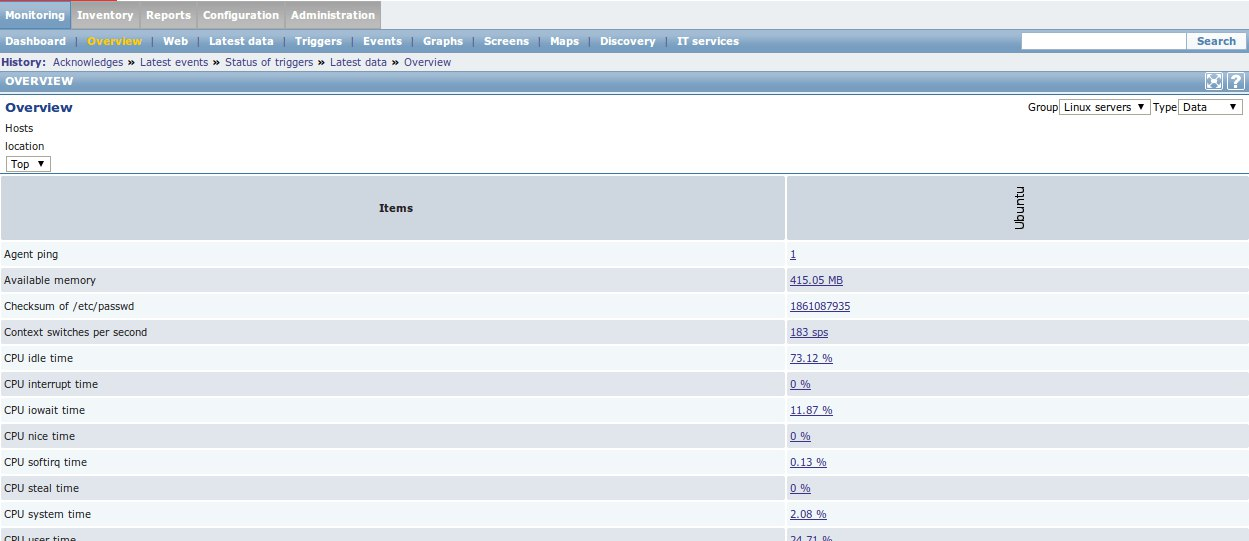
\includegraphics[width=0.8\linewidth]{eco/images/zbx.jpg}}
\caption{Просмотр данных о сервере}
\end{figure}